\chapter{Программая реализация разработанного метода нечеткого вывода с применением технологии CUDA}\label{ch:ch3}

Согласно схемам \cite{} изображенным в предыдущем разделе, для достижения высокой производительности процедура нечеткого вывода может быть скомпонована из последовательности параллельных участков независимых вычислений и сверток. Распространенным подходом реализации параллельных выччислений является использование вычислений на графическом процессоре.

Для удобства реализация выполнялась не постредством прямого использованием API библиотеки CUDA, а с помощью библиотеки реализации высокопроизводительных вычислений - \textbf{Kokkos} \cite{KokkosWiki, KokkosCarterEdwards20143202}, предназначенной для портативного и эффективного параллельного программирования на различных аппаратных архитектурах, включая многоядерные процессоры, графические процессоры NVIDIA/AMD и другие ускорители. Интерфейс библиотеки позволяет абстрагироваться от деталей низкоуровневого параллелизма, позволяя разработчикам писать код на C++ с одним исходным кодом, который может быть оптимизирован для различных платформ без существенных изменений. 
Ключевые функциональные возможности библиотеки упростившие выполнение программного реализации разработанного ранее метода:
\begin{itemize}
\item Модели параллельного выполнения: абстрагирование параллельных циклов (например, \lstinline{parallel_for}, \lstinline{parallel_reduce}) и рабочих процессов на основе задач.  
\item Управление памятью: Автоматизированная обработка пространств памяти (например, между хостом и устройством) и расположением данных для оптимизации схем доступа и минимизации объема передаваемых данных.  
\item Поддержка серверной части: интеграция с такими моделями программирования, как CUDA, HIP, OpenMP и SYCL, для обеспечения кроссплатформенной совместимости.  
\item Переносимость производительности: Обеспечивает эффективное использование ресурсов (потоки, векторизация) с учетом особенностей каждой архитектуры.
\end{itemize}

Kokkos широко используется в научных вычислениях и HPC-приложениях, упрощая разработку масштабируемых кодов при сохранении производительности на постоянно развивающемся оборудовании. 

При выполнении процедуры нечеткого вывода для набора входных данных можно выполнять процедуру вывода по каждому входному экземпляру независимо, то есть параллельно. Кроме того, можно предусмотреть отбор небольшого в сравнении с общим количеством ограниченного подмножества правил нечеткой системы, наиболее релевантных входному экземпляру. Сам алгоритм нечеткого вывода не предусматривает наличия промежуточной информации, которой бы нужно было обмениваться между вычислениями по другим экземплярам входных данных. Тогда, поскольку алгоритм нечеткого вывода для каждого экземпляра входных данных можно реализовать при ограниченном небольшом объеме входных и промежуточных данных, имеет смысл разместить эти данные в памяти предоставляющей наибольшую скорость доступа к данным, которая в технологии CUDA соответствует разделяемой памяти внутри CUDA-блока, а сами вычисления над этими данными также реализовать внутри этого CUDA-блока.

Из описанного выше функционала библиотеки Kokkos для размещения и доступа к данным в разделяемой памяти CUDA-блока крайне удобно использовать \lstinline{Kokkos::View} с опорой на широко эксплуатируемую в среде C++ разработчиков идиому RAII (Resource acquisition is initialization --- получение некоторого ресурса неразрывно совмещается с инициализацией, а освобождение --- с уничтожением объекта), которая позволяет избавиться от необходимости <<ручного>> вычисления адресов и смещений, располагаемых в разделяемой памяти, программых объектов, что особенно актуально при переиспользовании сегментов разделяемой памяти, занимаемых временными данными, в дальшейших шагах алгоритма.

Для удобства \dots

\begin{lstlisting}[language=C++]
using ScratchSpace =
	typename Kokkos::Cuda::scratch_memory_space;
template <typename DataType>
using ScratchView =
	Kokkos::View<DataType,
							 ScratchSpace,
							 Kokkos::MemoryTraits<Kokkos::Unmanaged>>;
\end{lstlisting}

Для выделения памяти c помощью \lstinline{Kokkos::View} требуется получить дескриптор разделяемой памяти текущего CUDA-блока с помощью вызова \lstinline{Kokkos::TeamHandleConcept<>::team_shmem()} , который описывает всю карту разделяемой памяти данного CUDA-блока. 

При оценке объема разделяемой памяти, необходимой для размещения данных внутри CUDA-блока. Рациональное использование только необходимого объема разделяемой памяти позволит планировщику на графическом процессоре поставить на исполнение сразу несколько CUDA-блоков на один \textit{потоковый мультипроцессор} (\textit{streaming multiprocessor}).

Вычисления в рамках нити

Поскольку вычисление свертки НЗИ для всех правил нечеткой системы составляет половину сложности алгоритма нечеткого вывода и в последствии будет неоднократно использооваться при агрегации правил, необходимо обеспечить единоразовое вычисление функции принадлежности свертки НЗИ (или ее аппроксимации), в результате которого будут известны значения последней на всей ее области определения.

\section{Вычисление нечеткого значения истинности посредством дискретизации}\label{sec:ch3/sect1}

При реализации вычисления НЗИ, когда функции принадлежности нечетких множеств $A$ и $A'$ заданы гауссовыми функциями, может возникнуть сложность, когда ф. п. НЗИ вырождается в близкий к некоторой асимптоте (горизонтальной или вертикальной) вид. Для изучения условий возникновения таких ситуаций перепишем формулу (\ref{eqn:ftv-gauss-expanded}) ниже и обозначим ее составные компоненты через $\alpha$, $\beta$, $\phi(v)$:
\begin{equation*}
	\exp\left(-\left(\underbrace{\frac{a_1-a_2}{b_2}}_{\alpha}\pm\underbrace{\frac{b_1}{b_2}}_{\beta}\underbrace{\sqrt{-\ln v}}_{\phi(v)}\right)^2\right).
	\label{eqn:ftv-gauss-components-markup}
\end{equation*}
Тогда вычисление значения (\ref{eqn:ftv-gauss-expanded}) можно представить в виде композиции функций
\begin{equation}
	\mu_{CP(A,A')}(v)=\exp(-z(v)^2),
	\label{eqn:ftv-gauss-exp-z}
\end{equation}
и
\begin{equation}
	z(v)=\alpha \pm \beta \phi(v).
	\label{eqn:ftv-gauss-phi}
\end{equation}

\pgfplotsset{
	membership axes/.style={
		%width=0.45\textwidth,
		%height=0.45\textwidth,
		scale only axis,
		domain=0:1,
		samples=100,
		every axis plot/.append style={smooth},
		axis lines=middle,
		xmin=0, xmax=1,
		ymin=0, ymax=1,
		xticklabel style={font=\tiny, inner sep=1pt, outer sep=0pt},
		yticklabel style={font=\tiny, inner sep=1pt, outer sep=0pt},
		legend style={font=\small},
	}
}


\begin{figure}[ht]
	\centering
	\begin{minipage}[t]{0.48\textwidth}
		\centering
		\begin{tikzpicture}
			\begin{axis}[
				membership axes,
				domain=0:5,
				samples=100,
				xmax=5,
			]
				\addplot [blue, thick] {exp(-(x^2))};
			\end{axis}
		\end{tikzpicture}
		\caption{График функции $\exp(-z^2)$}
		\label{fig:ftv-exp-component}
	\end{minipage}
	\hfill
	\begin{minipage}[t]{0.48\textwidth}
		\centering
		\begin{tikzpicture}
			\begin{axis}[
				membership axes,
				samples=100,
				ymax=3,
			]
				\addplot [blue, thick] {sqrt(-ln(x))};
			\end{axis}
		\end{tikzpicture}
		\caption{График функции $\phi(v)=\sqrt{-\ln v}$}
		\label{fig:ftv-phi-component}
	\end{minipage}
\end{figure}

Для иллюстрации условий возникновения описанных вырождений функции (\ref{eqn:ftv-gauss-expanded}) графики функций (\ref{eqn:ftv-gauss-exp-z}) и (\ref{eqn:ftv-gauss-phi}) при $\alpha = \beta = 1$ приведены на рисунках \cref{fig:ftv-exp-component} и \cref{fig:ftv-phi-component} соответственно. Из рисунка \cref{fig:ftv-phi-component} видно, что вырождение выражения (\ref{eqn:ftv-gauss-exp-z}) в близкий к асимптоте вид возможно при очень больших или очень малых значениях $\alpha$ и $\beta$. Данное наблюдение проиллюстрировано на рисунке \cref{fig:ftv-gauss-corner-cases}.

\begin{figure}[htbp]
	\centering
	
	% First row
	\begin{subfigure}[t]{0.48\textwidth}
		\newcommand{\aOne}{1}
		\newcommand{\bOne}{0.2}
		\newcommand{\aTwo}{0.95}
		\newcommand{\bTwo}{1}
		\centering
		\begin{tikzpicture}
			\begin{axis}[
				membership axes,
				samples=1000,
			]
				\addplot [blue, thick] {gauss(\aOne-2*\bOne*sqrt(-ln(x)), \aTwo, \bTwo)};
				\draw [blue, thick] (0.001464278918,0.8) -- (0.0001,0);
			\end{axis}
		\end{tikzpicture}
		\caption{$\mu_{CP(A, A')}(v)$ при $\alpha \approx 0, \beta \approx 0$}
		\label{fig:ftv-corner-cases-zeroBeta-1}
	\end{subfigure}
	\hfill
	\begin{subfigure}[t]{0.48\textwidth}
		\newcommand{\aOne}{1}
		\newcommand{\bOne}{1}
		\newcommand{\aTwo}{0.95}
		\newcommand{\bTwo}{0.1}
		\centering
		\begin{tikzpicture}
			\begin{axis}[
				membership axes,
				samples=1000,
			]
				\addplot [blue, thick] {gauss(\aOne-2*\bOne*sqrt(-ln(x)), \aTwo, \bTwo)};
			\end{axis}
		\end{tikzpicture}
		\caption{$\mu_{CP(A, A')}(v)$ при $\alpha \approx 0, \beta \gg 0$}
		\label{fig:ftv-corner-cases-largeBeta-1}
	\end{subfigure}
	
	% Second row
	\begin{subfigure}[t]{0.48\textwidth}
		\newcommand{\aOne}{3.34}
		\newcommand{\bOne}{0.02}
		\newcommand{\aTwo}{5}
		\newcommand{\bTwo}{1}
		\centering
		\begin{tikzpicture}
			\begin{axis}[
				membership axes,
				samples=1000,
				domain=0.001:1,
			]
				\addplot [blue, thick] {gauss(\aOne+2*\bOne*sqrt(-ln(x)), \aTwo, \bTwo)};
			\end{axis}
		\end{tikzpicture}
		\caption{$\mu_{CP(A, A')}(v)$ при $|\alpha| \gg 0, \beta \approx 0$}
		\label{fig:ftv-corner-cases-zeroBeta-2}
	\end{subfigure}
	\hfill
	\begin{subfigure}[t]{0.48\textwidth}
		\newcommand{\aOne}{3.34}
		\newcommand{\bOne}{1}
		\newcommand{\aTwo}{5}
		\newcommand{\bTwo}{0.02}
		\centering
		\begin{tikzpicture}
			\begin{axis}[
				membership axes,
				samples=1000,
				domain=0.001:1,
			]
				\addplot [blue, thick] {gauss(\aOne+2*\bOne*sqrt(-ln(x)), \aTwo, \bTwo)};
			\end{axis}
		\end{tikzpicture}
		\caption{$\mu_{CP(A, A')}(v)$ при $|\alpha| \gg 0, \beta \gg 0$}
		\label{fig:ftv-corner-cases-largeBeta-2}
	\end{subfigure}
	
	% Third row
	\begin{subfigure}[t]{0.48\textwidth}
		\newcommand{\aOne}{1}
		\newcommand{\bOne}{0.1}
		\newcommand{\aTwo}{0.3}
		\newcommand{\bTwo}{0.1}
		\centering
		\begin{tikzpicture}
			\begin{axis}[
				membership axes,
				samples=1000,
			]
				\addplot [blue, thick] {gauss(\aOne-2*\bOne*sqrt(-ln(x)), \aTwo, \bTwo)};
				\draw [blue, thick] (0.0014,0.4) -- (0.0001,1);
			\end{axis}
		\end{tikzpicture}
		\caption{$\mu_{CP(A, A')}(v)$ при $|\alpha| \gg 0, \beta = 1$}
		\label{fig:ftv-corner-cases-oneBeta}
	\end{subfigure}
	
	\caption{Случаи вырождения ф. п. НЗИ в близкий к асимптоте вид.}
	\label{fig:ftv-gauss-corner-cases}
\end{figure}

В ситуациях, изображенных на рисунках \cref{fig:ftv-corner-cases-zeroBeta-1, fig:ftv-corner-cases-largeBeta-1, fig:ftv-corner-cases-largeBeta-2, fig:ftv-corner-cases-oneBeta}, функция принадлежности НЗИ имеет своей асимптотой вертикальную прямую $v = v_0$. При реализации вычисления НЗИ с использованием расчетной сетки, связанная с тем, что ф. п. НЗИ в точке может быть вообще не определена (рис. \cref{fig:ftv-corner-cases-zeroBeta-1, fig:ftv-corner-cases-oneBeta}) или ф. п. НЗИ в точке $v_0$ имеет значение сильно отличающееся от значений в ближайших точках расчетной сетки $v_1$ и $v_2$ при $v_0 \in (v_1, v_2)$, из-за чего значение НЗИ в бесконечно малой окрестности точки $v_0$ будет упущено.

Из рисунка \cref{fig:ftv-exp-component} видно, что максимальное значение выражения (\ref{eqn:ftv-gauss-exp-z}), равное 1, достигается при $z = 0$, а из рисунка \cref{fig:ftv-phi-component} видно, что функция (\ref{eqn:ftv-gauss-phi}) обязательно пересекает ось абсцисс, то есть максимальное значение ф. п. НЗИ всегда равно 1. Тогда для решения проблемы <<просеивания>> значения $\mu_{CP(A, A')}(v_0)$ сквозь точки расчетной сетки можно вычислить координату точки $v_0$, в которой функция (\ref{eqn:ftv-gauss-expanded}) принимает свое максимальное значение, а затем положить значение в ближайшей к $v_0$ точке расчетной сетки равным этому максимуму, то есть значению 1. Для этого выразим аналитически значение $v_0$, в котором (\ref{eqn:ftv-gauss-expanded}) принимает значение 1.

\begin{align}
	\exp\left(-\left(\frac{(a_1-a_2)\pm b_1\sqrt{-\ln v_0}}{b_2}\right)^2\right) &= 1 \nonumber \\
	\exp\left(-\left(\frac{(a_1-a_2)\pm b_1\sqrt{-\ln v_0}}{b_2}\right)^2\right) &= \exp(0) \nonumber \\
	\frac{(a_1-a_2)\pm b_1\sqrt{-\ln v_0}}{b_2} &= 0 \nonumber \\
	\pm b_1\sqrt{-\ln v_0} &= a_1-a_2 \nonumber \\
	\sqrt{-\ln v_0} &= \pm\frac{a_1-a_2}{b_1} \nonumber \\
	\ln v_0 &= -\left(\frac{a_1-a_2}{b_1}\right)^2 \nonumber \\
	v_0 &= \exp\left(-\left(\frac{a_1-a_2}{b_1}\right)^2\right) \label{eqn:ftv-gauss-argmax}
\end{align}

Внедрение выражения (\ref{eqn:ftv-gauss-argmax}) в алгоритм вычисления НЗИ позволит обеспечить соответствие определению дискретизированного представления ф. п. НЗИ. \todo{Строго говоря ф. п. на рисунке определена в точке $v_0$ и не требует\dots.} НЗИ с функцией принадлежности, имеющей горизонтальную асимптоту, как на рисунке \cref{fig:ftv-corner-cases-zeroBeta-2} может вызвать сложность при построении алгоритма вычисления НЗИ на использовании метода градиентного спуска вместо дискретизации с фиксированным шагом расчетной сетки.

Вычисление нечеткого значения истинности для каждого правила по каждому входу отдельно предварительным этапом приведет к линейному увеличению объема необходимой памяти. Поскольку вычисление НЗИ является довольно легкой операцией, лучшим решением будет встраивание вычисления НЗИ по каждому входу в процедуру свертки НЗИ.

Формула (\ref{}) предлагает построение процедуры свертки НЗИ в виде дерева попарных сверток, для сохранения промежуточных результатов которых потребуется выделение объема памяти, также имеющего фактически линейный порядок зависимости от количества входов нечеткой системы. Возвращаясь к формуле (\ref{}) свертки НЗИ по входам в [] предложен параллельный алгоритм свертки НЗИ на расчетной сетке с постоянным шагом. Данный алгоритм итеративно вычисляет значение светки НЗИ в каждой точки расчетной сетки продвигаясь от точки в пространстве истинности 1 к точке 0. Для каждого правила отдельно потребуется объем памяти, необходимый для сохранения значений свертки НЗИ в каждой точке расчетной сетки и для сохранения текущего максимального значения НЗИ по каждому входу на данной итерации алгоритма.

Преимуществом такого подхода представления НЗИ в программе является возможность быстрого нахождения значения функции принадлжености НЗИ в некоторой точке пространства истинности. Пара ближайших к этой точке позиций в массиве значений НЗИ на расчетной сетке определяется на основе значения фиксированного шага расчетной сетки. Для вычисления непосредственно ззначения НЗИ используется линейная интерполяция для найденной пары.

Поскольку при небольшом количестве входных переменных нечеткой системы большие участки расчетной сетки ф. п. светки НЗИ соответствуют ф. п. НЗИ по одному из входов, при том же объеме памяти, необходимой для хранения результа сверки НЗИ, можно перейти к переменному шагу расчетной сетки с увеличением сложности функции аппроксимации участков ф. п. свертки НЗИ, принадлежащий ф. п. НЗИ одного из входов. Схема вычислений такого алгоритма схожа со схемой алгоритма при использовании постоянного шага расчетной сетки, а на каждой итерации определяется точка \dots

\begin{figure}[ht]
	\centering
	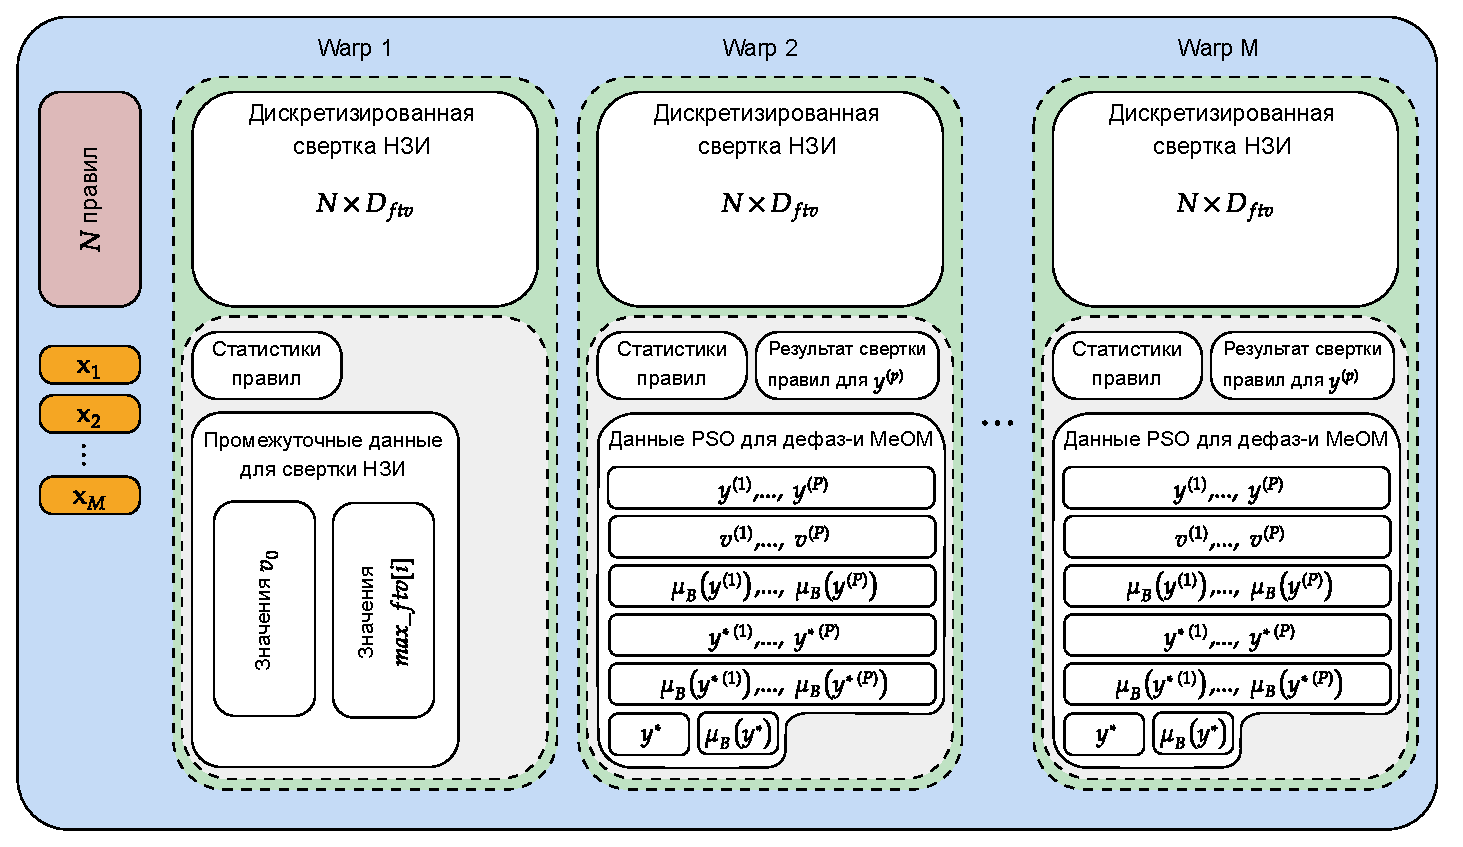
\includegraphics[scale=0.7]{cuda-shared-memory-map}
	\caption{Карта разделяемой памяти одного CUDA-блока нечеткого логического вывода на основе нечеткого значения истинности при использовании дефаззификации MeOM.}
	\label{fig:ftv-infer-cuda-shared-memory-map}
\end{figure}

Ввиду необходимости использования большой размерности расчетной сетки для получения высокой точности дискретизации для размещения результата свертки НЗИ потребуется существенный объем разделяемой памяти. Например, при использовании для задания вычисленных значений вещественных чисел одинарной точности (4 байта) и размерности расчетной сетки равной 100 сохранение результата свертки НЗИ в нечеткой системе с 50 правилами в базе правил потребуется $4\textrm{ байта}\times 100 \times 50 = 20000\textrm{ байт}$ разделяемой памяти. Согласно документации CUDA, устройства с \textit{набором вычислительных возможностей} (\textit{compute capabilities}) версии 7.5 (и некоторых более низких версий) максимальный объем разделяемой памяти на одном потоковом мультипроцессоре равен 64 Кб, а на устройствах с набором вычислительных возможностей более высокой версии --- предусмативается 100 - 164 Кб разделяемой памяти. Следовательно время нечеткого вывода может быть сокращено за счет сокращения времени работы отдельного CUDA-блока путем увеличения количества нитей. Однако с другой стороны слишком большое количество нитей внутри CUDA-блока упрется в ограниченное количество ригистровой памяти и ограниченное количество арифметико-логических модулей внутри потокового мультипроцессора (распределяемых между нитями 4-мя планировщиками на большинстве версий наборов вычислительных возможностей).

\begin{figure}[hbt]
	\centering
   	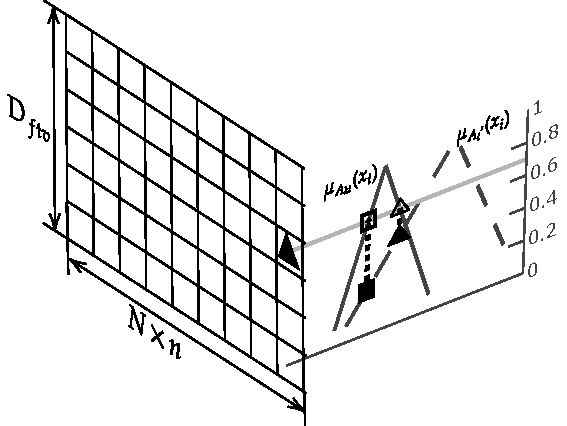
\includegraphics[width=0.6\textwidth]{ftv-opengl-computation.pdf}
	\label{ftv-opengl-computation}
\end{figure}

\begin{figure}[hbt]
	\centering
   	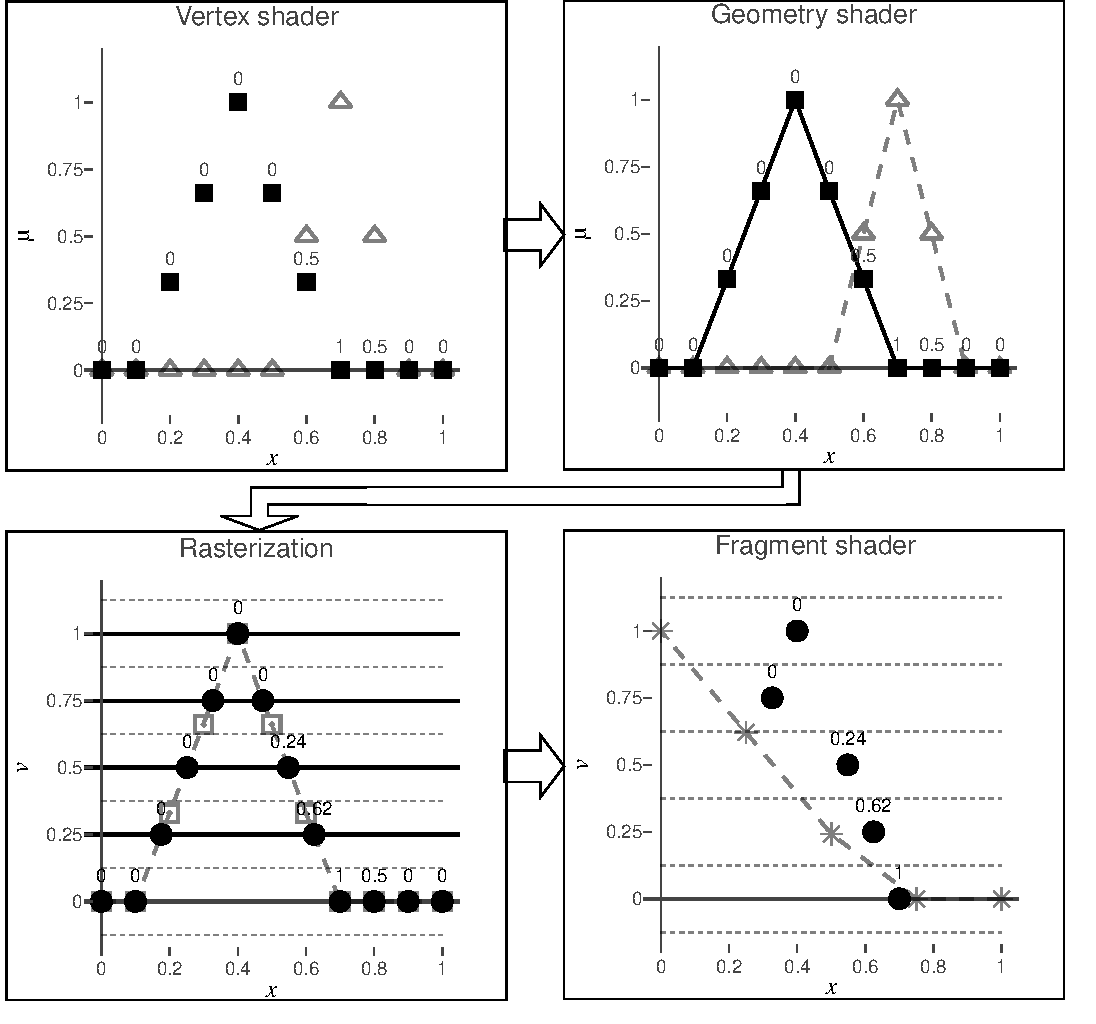
\includegraphics[width=1.0\textwidth]{ftv-opengl-computation-pipeline.pdf}
	\label{ftv-opengl-computation-pipeline}
\end{figure}

\section{Алгоритм свертки НЗИ при $T_1=min$ и $T_3$ - неубывающая по всем аргументам}\label{sec:ch3/sect2}

При дискретизированном вычисление ф. п. свертки НЗИ в некоторой точке расчетной сетки $v_j\in [0,1]$ потребуется просматривать значения НЗИ в отрезке $[v_j, 1]$, то есть имеет вычислительную сложность $O(D_{ftv})$, где $D_{ftv}$ --- число точек расчетной сетки ф. п. НЗИ. Таким образом вычисление свертки НЗИ по формуле (\ref{eqn:ftv-compute-11}) может быть распараллелено по точкам расчетной сетки, а нахождение $\tau_{\mathbf{A_k}|\mathbf{A'}}(v_j)$ использует операцию свертки, которая в имеет ограниченную возможность распараллеливания, но в целом требует большого количества повторных вычислений значений $\tau_{A_{ki}|A'_i}(v_k), v_k\in [v_j, 1]$. В \cite{Karatach2024} предложен алгоритм вычисления свертки НЗИ сразу по всем входам с использованием техники динамического программирования, имеющий линейную зависимость от размера расчетной сетки $D_{ftv}$. Алгоритм приведен на \cref{alg:ftv-reduction}.

\begin{algorithm}
\begin{algorithmic}
\Require $ftv_i,\ i=\overline{1,n}$
\State $max\_ftv[i] = 0;$
\For{$v_j = 1\dots0$}
\State $s \gets \left\{ftv_i[v_j] \mid ftv_i[v_j] >= max\_ftv[i]\right\};$
\State $max\_ftv[i] \gets max(max\_ftv[i], ftv_i[v_j]);$
\State $v\_max \gets \max_{i}\left\{ftv_i[v_j]\right\}, v\_max\_index \gets \mathrm{arg\,max}_i\left\{ftv_i[v_j]\right\};$
\If{$s = \emptyset \And i = v\_max\_index$}
\State $r[i] \gets v\_max;$
\Else
\State $r[i] \gets max\_ftv[i];$
\EndIf
\State $ftv'[v_j] \gets \underset{i}{T_3}\left\{r[i]\right\}$;
\EndFor
\State \Return $ftv'$
\end{algorithmic}
\caption{Алгоритм свертки НЗИ при $T_1=min$ и $T_3(a, b) \ge T_3(c, d)$ если $a > c$ или $b > d$}
\label{alg:ftv-reduction}
\end{algorithm}

Данный алгоритм итеративно вычисляет значения $\tau_{\mathbf{A_k}|\mathbf{A'}}(v_j)$, продвигаясь от точки $v_j = 1$ к $v_j = 0$. При этом распараллеливаются вычисления по $n$ входам. В $i$-х элементах массива $max\_ftv$ хранятся максимальные значения $\tau_{A_{ki}|A'_i}(v_k)$ для $j$-й итерации, что избавляет от необходимости поиска этих значений на каждой итерации. Также, поскольку на $j$-й итерации значение $\tau_{\mathbf{A_k}|\mathbf{A'}}(v_j)$ выражается из значений НЗИ по входам в точках $v_{ki}, i=\overline{1,n}$, то, с учетом ограничения алгоритма $T_1 = min$ и согласно выражению из формулы (\ref{eqn:ftv-compute-8})
\[
\underset{i=\overline{1,n}}{\mathrm{T_1}}v_{ki} = v_j,
%\sup_{\substack{\underset{i=\overline{1,n}}{\mathrm{T_1}}v_i = v \\ (v_1, \dots, v_n) \in [0, 1]^n}} \left\{\underset{i=\overline{1,n}}{\mathrm{T_3}}\tau_{A_{ki}|A'_i}(v_i)\right\}
\]
для одного из значений $v_{ki}$ необходимо выполнение $V_{ki} = v_j$. Для этого в \cref{alg:ftv-reduction} используется максимальное значение $\tau_{A_{ki}|A'_i}(v_j), i=\overline{1,n}$, когда ни по одному входу не обнаружено нового максимума ф. п. НЗИ в точке $v_j$.

Для лучшего понимания работу алгоритма на каждой итерации можно представить с помощью диаграммы <<роза ветров>> с количеством осей равным $n$, в центре диаграммы находится координата осей равная 1, а сама <<роза>> проходит через текущие максимумы ф. п. НЗИ на отрезке $[v_j, 1]$.

\begin{figure}[ht]
	\centering
	\begin{tikzpicture}[scale=5]
		% Parameters
		\def\n{6}
		\def\step{72} % 360/5
		\def\totalRadius{1.0}
		\def\currentRadius{0.5}
		\def\radiusOffset{0.1}
		% Function values for each direction
		\def\maxFtvYA{0.9},%
		\def\maxFtvYB{0.4},%
		\def\maxFtvYC{0.9},%
		\def\maxFtvYD{0.6},%
		\def\maxFtvYE{0.4},%
		\def\maxFtvYF{1.0}

		\def\maxFtvXA{1.0},%
		\def\maxFtvXB{0.5},%
		\def\maxFtvXC{1.0},%
		\def\maxFtvXD{1.0},%
		\def\maxFtvXE{0.5},%
		\def\maxFtvXF{1.0}

		% Angles for each direction
		\foreach \i/\angle in {1/90,2/30,3/330,4/270,5/210,6/150} {
			% Draw direction lines
			\draw[gray!40] ({(\radiusOffset)*cos(\angle)},{(\radiusOffset)*sin(\angle)}) -- ({(\radiusOffset+\totalRadius)*cos(\angle)},{(\radiusOffset+\totalRadius)*sin(\angle)});
			\node[font=\small] at ({(2*\radiusOffset+\totalRadius)*cos(\angle)},{(2*\radiusOffset+\totalRadius)*sin(\angle)}) {$0$};
		}
		% Draw base circle
		\draw[gray!50] (0,0) circle (\radiusOffset);
		\draw[gray!50] (0,0) circle (\radiusOffset+\totalRadius);
		\node[font=\small] at (0,0) {$1$};
		
		% Connect the top points to form the rose in the horizontal plane at z=0
		\coordinate (A) at ({(\radiusOffset+1-\maxFtvXA)*cos( 90)},{(\radiusOffset+1-\maxFtvXA)*sin( 90)});
		\coordinate (B) at ({(\radiusOffset+1-\maxFtvXB)*cos( 30)},{(\radiusOffset+1-\maxFtvXB)*sin( 30)});
		\coordinate (C) at ({(\radiusOffset+1-\maxFtvXC)*cos(330)},{(\radiusOffset+1-\maxFtvXC)*sin(330)});
		\coordinate (D) at ({(\radiusOffset+1-\maxFtvXD)*cos(270)},{(\radiusOffset+1-\maxFtvXD)*sin(270)});
		\coordinate (E) at ({(\radiusOffset+1-\maxFtvXE)*cos(210)},{(\radiusOffset+1-\maxFtvXE)*sin(210)});
		\coordinate (F) at ({(\radiusOffset+1-\maxFtvXF)*cos(150)},{(\radiusOffset+1-\maxFtvXF)*sin(150)});
%		\coordinate (A) at ({\maxFtvX[0]*cos(90)},{\maxFtvX[6]*sin(90)});
%		\coordinate (B) at ({0.5*cos(30)},{0.5*sin(30)},0.4*\zstep*0);  % ftv_2[3]
%		\coordinate (C) at ({1.0*cos(330)},{1.0*sin(330)},0.9*\zstep*0);% ftv_3[0]
%		\coordinate (D) at ({1.0*cos(270)},{1.0*sin(270)},0.6*\zstep*0);% ftv_4[0]
%		\coordinate (E) at ({1.0*cos(210)},{1.0*sin(210)},0.4*\zstep*0);% ftv_5[4]
%		\coordinate (F) at ({1.0*cos(150)},{1.0*sin(150)},1.0*\zstep*0);% ftv_6[0]
		\draw[thick,red,fill=red,fill opacity=0.15]
			(A) -- (B) -- (C) -- (D) -- (E) -- (F) -- cycle;
		
		\draw[blue!60] (0,0) circle (\radiusOffset+\currentRadius);
		% Optionally, label directions
		\foreach \angle/\lbl/\x/\y in {
			90/1/\maxFtvXA/\maxFtvYA,
			30/2/\maxFtvXB/\maxFtvYB,
			330/3/\maxFtvXC/\maxFtvYC,
			270/4/\maxFtvXD/\maxFtvYD,
			210/5/\maxFtvXE/\maxFtvYE,
			150/6/\maxFtvXF/\maxFtvYF} {
			\node[font=\small,pin={[pin distance=1cm] \y}] at ({(\radiusOffset+\currentRadius)*cos(\angle)},{(\radiusOffset+\currentRadius)*sin(\angle)},0) {$\mathrm{max\_ftv}_{\lbl}=\y$};
		}
	\end{tikzpicture}
	\caption{3D wind rose diagram for 6 directions with function values plotted vertically.}
	\label{fig:wind-rose-3d}
\end{figure}

\begin{figure}
    \label{fig:ftvs-reduction-example}
    \centering
    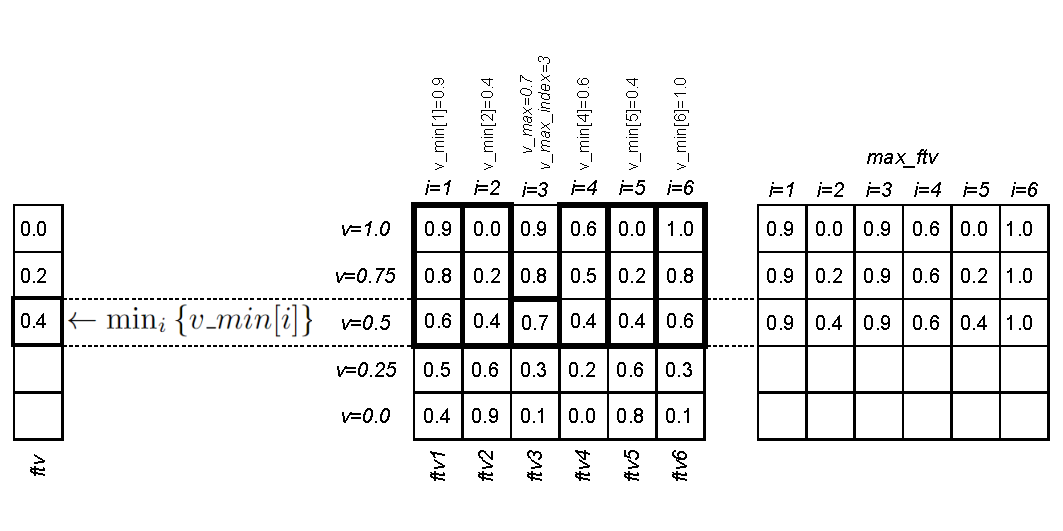
\includegraphics[width=15cm]{ftvs-reduction-example.pdf}
    \caption{Иллюстрация работы алгоритма свертки НЗИ для нескольких входов для расширенной $\mathrm{\tilde{T}}$-нормы при $T_1=\mathrm{min}$ и $T_3=\mathrm{min}$.}
\end{figure}

При 

\pgfplotsset{
    axis grid/.style={
        width=0.3\textwidth,
        height=0.3\textwidth,
        domain=0:1,
    }
}


\section{Реализация дефаззификации}

Производительность дефаззификации по \textit{упрощенной схеме метода COG} может быть увеличена путем масштабирования вычислений внутри блока по центрам выходной лингвистической переменной.

Поскольку используемые в данной работе в качестве функций принадлежности гауссовы функции являются гладкими во всей области определения выходной лингвистической переменной, для точного нахождения максимального значения ф. п. выходного нечеткого множества при дефаззификации по \textit{методу среднего максимума (MeOM)} можно использовать алгоритм градиентного спуска. В ситуации когда вычисление значения агрегированной по всем правилам выходной функции принадлежности и ее производных в некоторой точке выходного пространства является вычислительно сложной процедурой, целесообразно будет использовать \textit{метод Ньютона второго порядка} для более быстрого нахождения точки максимума выходной ф. п.:
\begin{equation}
	y^{(k+1)} = y^{(k)} - \alpha \frac{\mu_{B'}^{'}(y^{(k)})}{\mu_{B'}^{''}(y^{(k)})},
	\label{eqn:defuz-impl-meom-1}
\end{equation}
где $\alpha $ - коэффициент шага градиента.

Сложность может составить вопрос инициализации начальной координаты точки $y^{(0)}$, ведь в отдаленных от точки максимума выходной ф. п. $\mu_{B'}(y^{(0)})$  соответствующая ее минимуму гауссова функция может принять горизонтальный вид с нулевыми производными вне границ отрезка $[a_{B'} - 4 b_{B'}, a_{B'} + 4 b_{B'}]$. Для получения начального приближения можно использовать вычислительно более простой метод дефаззификации, например, дефаззификацию по методу среднего центра (CA). Также стоит добавить в формулу (\ref{eqn:defuz-impl-meom-1}) штраф за отдаление от точки $\hat{y}_{CA}$ с весовым параметром учета штрафа $\lambda$, а также учитывать штраф при низких значениях $\mu_{B'}(y^{(k)})$. С помощью параметра $\lambda$ и номера итерации $k$ можно обеспечить плавный сдвиг вклада в шаг итерации от штрафа до значения градиента с ростом числа прошедших итераций. Тогда формула (\ref{eqn:defuz-impl-meom-1}) примет вид:
\begin{gather*}
	y^{(k+1)} = y^{(k)} + \alpha \left(\mu_{B'}(y^{(k)})(1-\lambda)\left(-\frac{\mu_{B'}^{'}(y^{(k)})}{\mu_{B'}^{''}(y^{(k)})}\right) + (1-\mu_{B'}(y^{(k)}))\lambda (\hat{y}_{CA} - y^{(k)})\right),\\
	\lambda = e^{-k \gamma},
	\label{eqn:defuz-impl-meom-2}
\end{gather*}
где хорошая сходимость алгоритма показывается при выборе для параметра $\gamma$ значения равного коэффициенту шага $\alpha$.

Для преодоления проблемы локальных максимумов выходной функции принадлежности (которые ожидаемо возникнут при использовании $t$-нормы минимума или произведения для агрегации гауссовых функций) и сглаживания линии градиента, распространенной практикой является добавление момента $v^(k)$ в алгоритм градиентного спуска:
\begin{gather}
\begin{split}
	v^{(k+1)} = \omega v^{(k)} + (\mu_{B'}(y^{(k)})(1-\lambda)\left(-\frac{\mu_{B'}^{'}(y^{(k)})}{\mu_{B'}^{''}(y^{(k)})}\right) + (1-\mu_{B'}(y^{(k)}))\lambda (\hat{y}_{CA} - y^{(k)})),\\
	y^{(k+1)} = y^{(k)} + \alpha v^{(k+1)},
\end{split}
\label{eqn:defuz-impl-meom-3}
\end{gather}
где $\omega$ --- параметр скользящего среднего значения момента.

\begin{figure}[ht]
	\centering
	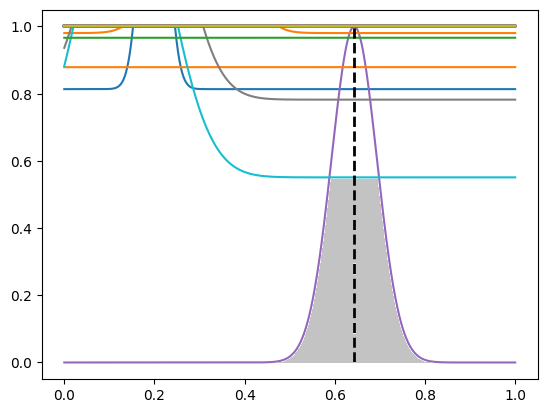
\includegraphics{meom-use-case.png}
	\caption{Ситуация необходимости нахождения среднего максимума при дефаззификации агрегированной функции принадлежности $\mu_{B'}(y)$.}
	\label{fig:defuz-meom-use-case}	
\end{figure}

Необходимость усреднения максимумов при использовании метода дефаззификации Mean of Maximum возникает в ситуации изображенной на рисунке \cref{fig:defuz-meom-use-case}, где истинное значение $y$ нарисовано пунктирной линией. Вычислить среднее значение $y$ можно как выборочное среднее. Получить такую выборку точек можно посредством многократной оптимизации описанном выше методом. Как и в случае с упрощенной схемой дефаззификации каждая такая оптимизация может происходить в отдельной группе нитей (warps) за счет масштабирования одного CUDA-блока.

Для этого можно использовать один из методов глобальной оптимизации, например, \textit{Gradient-aware Particle Swarm Optimizatiion}. Метод Particle Swarm Optimization (PSO) обеспечивает синхронизацию информации о текущей глобальной точке оптимума на данной итерации внутри популяции точек, что сокращает число итерации до сходимости к максимальному значению выходной функции принадлежности. С учетом (\ref{eqn:defuz-impl-meom-3}) для данного метода формулы шага оптимизации можно составить следующим образом:
\begin{align}
	\begin{split}
		v_i^{(k+1)} &= \omega v_i^{(k)} +\\
		&+ \alpha_l \left(
			r_l\left(
				y_i^{best} - y_i^{(k)}
			\right) + (1-r_l)\left(
				-\frac{\mu_{B'}^{'}(y_i^{(k)})}{\mu_{B'}^{''}(y_i^{(k)})}
			\right)
		\right) + \\
		&+ \alpha_g \left(
			r_g \mu_{B'}(y^{best})\left(
				y^{best}-y
			\right) + (1-r_g) \left(
				1-\mu_{B'}(y^{best})
			\right) \left(
				\hat{y}_{CA} - y^{(k)}
			\right)
		\right), \label{eqn:defuz-impl-meom-4-1}
	\end{split}\\
	y^{(k+1)} &= y^{(k)} + v^{(k+1)}, \nonumber
\end{align}
где $\alpha_l$ и $\alpha_g$ --- коэффициенты шага в направлении текущей точки локального и глобального оптимума, $r_l$ и $r_g$ --- случайно сгенерированные числа в диапазоне $[0,1]$, параметризующие движение в сторону текущих точек локального и глобального оптимума алгоритма PSO между движением в сторону роста градиента и точки начального приближения $\hat{y}_{CA}$ соответственно.

\begin{figure}[ht]
	\centering
	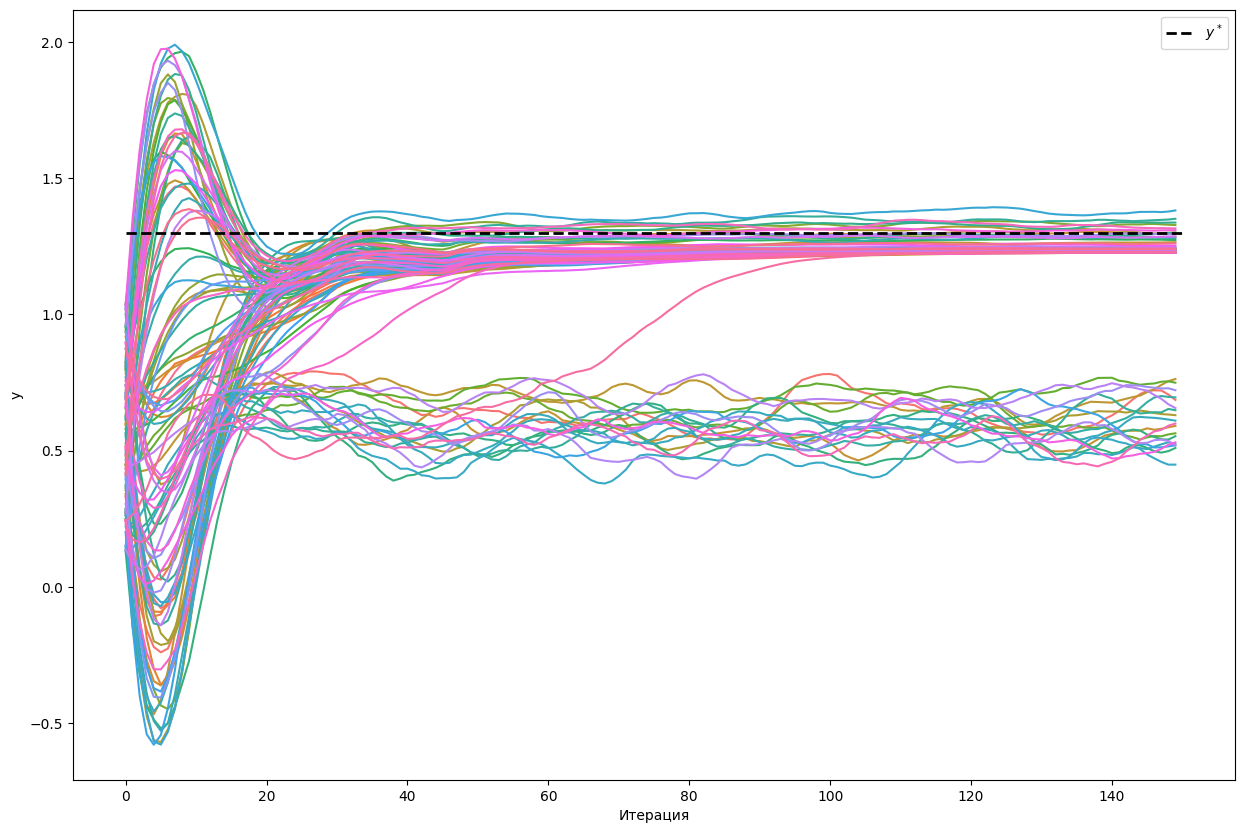
\includegraphics[scale=0.55]{defuz-meom-pos-hue.png}
	%	\hfill
	%	\begin{subfigure}{0.5\textwidth}
		%		\centering
		%		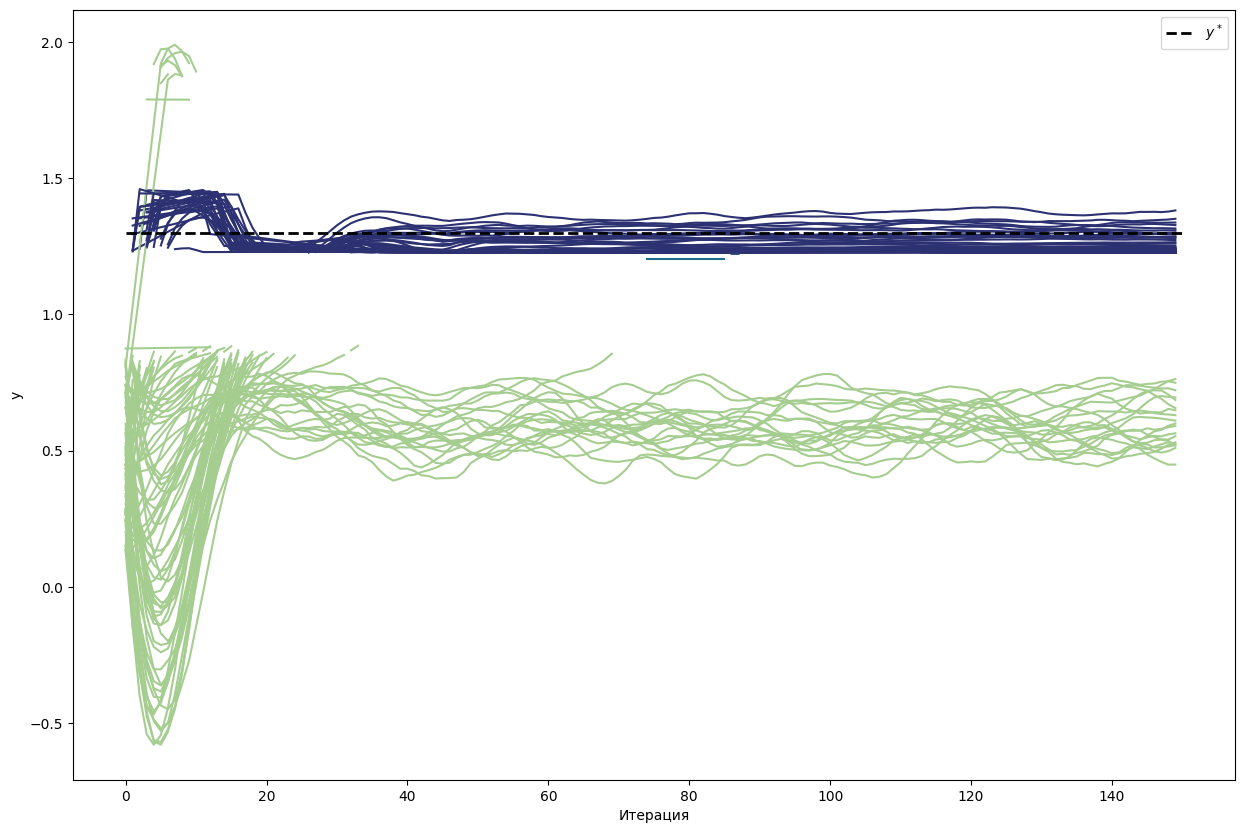
\includegraphics{defuz-meom-pos-brightness.png}
		%	\end{subfigure}
	\caption{Динамика движения точек популяции при работе алгоритма глобальной оптимизации Gradient-aware PSO.}
	\label{fig:defuz-meom-pso-hue}
\end{figure}

Компонента после коэффициента $\alpha_l$ в формуле (\ref{eqn:defuz-impl-meom-4-1}) обеспечить разнообразие среди точек популяции, достигших максимума $\mu_{B'}(y_i^{(k)})$. График работы такого алгоритма PSO приведен на рисунке \cref{fig:defuz-meom-pso-hue}. Как видно из него --- большинство точек популяции сосредоточились возле точки оптимума.

Для реализации дефаззификации по \textit{методу центра тяжести} можно использовать алгоритм оптимизации из предыдущего метода, сохраняя координаты $y_i^{(k)}$ и значения $\mu_{B'}(y_i^{(k)})$ на каждой итерации, а затем для вычисления формулы (\ref{eqn:defuz-cog-2}) использовать численное интегрирование, например, методом Симпсона.

\section{Использование библиотеки ArborX}\label{sec:ch3/sect2}

\begin{figure}[hbt]
	\label{fig:z-curve-apetrei}
	\centering
	\begin{minipage}[b]{0.45\textwidth}
		\centering
		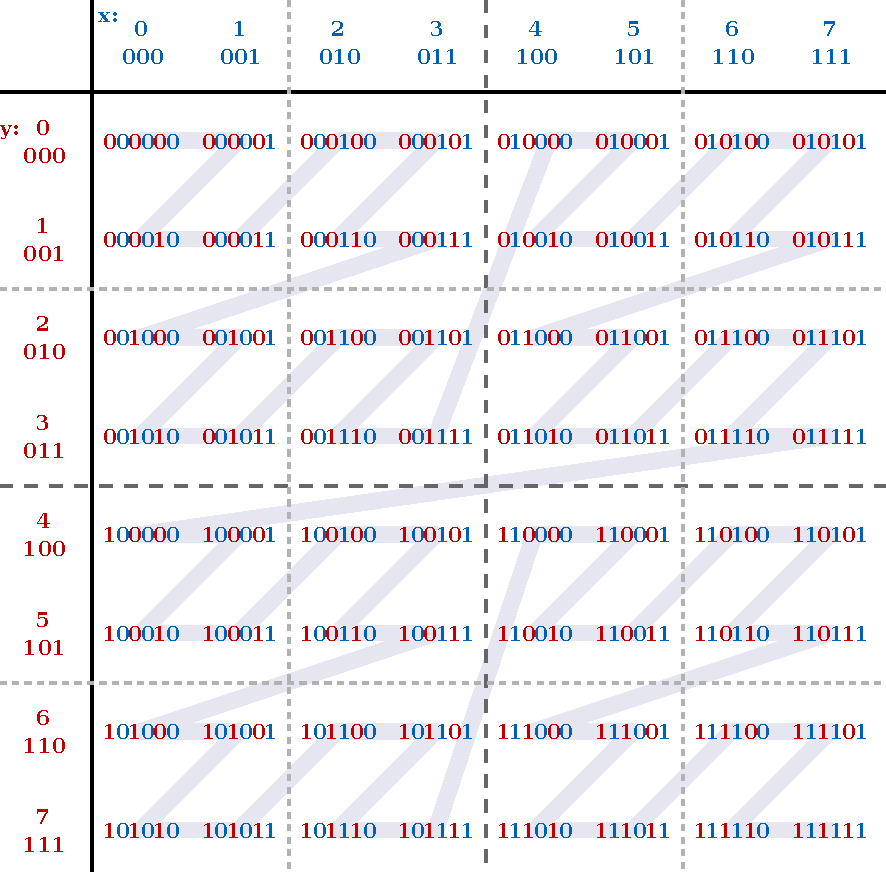
\includegraphics[width=\textwidth]{z-curve}
		\caption*{(a) z-curve}
	\end{minipage}\hfill
	\begin{minipage}[b]{0.45\textwidth}
		\centering
		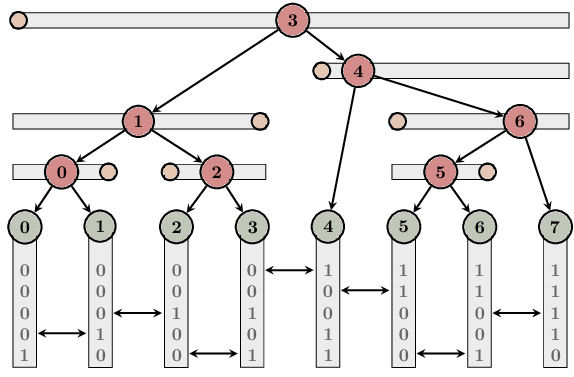
\includegraphics[width=\textwidth]{apetrei}
		\caption*{(b) apetrei}
	\end{minipage}
	\caption{Две иллюстрации: графика z-curve и apetrei.}
\end{figure}

В \cite{prokopenko2024revisingapetreisboundingvolume} авторами библиотеки \textbf{ArborX} предложен алгоритм для эффективного построения \textit{иерархии ограничивающих объемов}. Данная структура данных используется для эффективного поиска ближайшей точки в $n$-мерном пространстве. Алгоритм выполняет построение структуры поиска за $O(N\times log(N))$, где $N$ - количество точек в исходном наборе. Логика поиска места в иерархии ограничивающих объемов для каждой отдельной точки помещена в отдельную нить параллельных вычислений, после чего остается только логирифмическая компонента сложности, соответствующая восходящему обходу промежуточного дерева и помещения точки в подобранный узел \fixme{с использованием атомарной операции}. В основе алгоритма лежит группировка близко расположенных точек для более быстрого подбора соответствующего ограничивающего объема за счет проецирования точки из $n$-мерного пространства на $Z$-кривую посредством вычисления кода Мортона для каждой точки. Согласно эвристике, лежащие рядом на $Z$-кривой точки располагаются достаточно близко и исходном $n$-мерном пространстве. Кроме того в статье описан модифицированный алгоритм Апетрея [], обеспечивающий обход иерархии на этапе поиска ближайших точек без необходимости помещения цепочки пройденных родительских узлов в стек за счет передачи информации об альтернативных узлах-кандидатах из родительских узлов в дочерние. Такой подход значительно снижает количество потребляемой памяти для сохранения промежуточной информации при выполнении этапа поиска.

\section{Реализация алгоритма построения базы правил}

\section{Реализация обертки в Python-модуль}

Для ускорения процесса отладки и тестирования, выполненная на языке C++ (CUDA) реализация нечеткой модели собирается компилятором NVCC в динамически подключаемую библиотеку (\textit{*.so} (\textit{shared object}) файл в Linux). Реализованная на языке C часть Python-обертки библиотеки выполняет поиск файла библиотеки и символов в нем уже при запуске использующей эту библиотеку программы.

На сегодняшний день язык программирования Python занял позицию отраслевого стандарта в научных исследованиях и задачах анализа данных  Это обеспечено прежде всего удобным синтаксисом и легкостью интеграции большим многообразием высокопроизводительных библиотек научных вычислений, реализованных на языках с прямым управлением аппаратными ресурсами. Среди инструментов обеспечивающих реализацию механизма FFI в языке Python простым в использовании является инструмент Cython. Этот компилируемый метаязык расширяет парадигму Python, вводя статическую типизацию и структуры данных, характерные для системного программирования, что обеспечивает прозрачное описание C++ API. Современные инструменты пакетирования, включая обновленные версии setuptools, реализуют стандартизированные механизмы (PEP-517) для автоматизации включения Cython-компонентов в Python-пакеты.

\section{Выводы}

\begin{enumerate}
	\item 
\end{enumerate}

